%--------------------------------------------------------------------------------------------------
\chapter{Autonomous Data Cleaning on a Stream}
\label{ch:data-cleaning}
%--------------------------------------------------------------------------------------------------

%\epigraph{Everybody wants to save the Earth; no one wants to help mom do the dishes.}{\textit{P. J. O'Rourke}}
%\epigraph{You don't get anything clean without getting something else dirty.}{\textit{Cecil Baxter}}
\epigraph{Grabage in, garbage out.}{\textit{Gerorge Fuechsel}}

% introducing the paper
\begin{quote}
In this chapter, we introduce the paper entitled \textit{Autonomous Sensor Data Cleaning in a Stream Mining Setting}, authored by Klemen Kenda and Dunja Mladenić. 
This paper has been published in the Business Systems Research Journal~\cite{kenda:2018:autonomous}.
Klemen Kenda contributed to the conceptualization, methodology, software development, evaluation, and visualization.
Furthermore, he took the lead in writing the paper.
\end{quote}

% description of the scientific method
Data streams originating from the IoT are inherently prone to various inconsistencies and flaws.
Autonomous data cleaning engine is a prerequisite for an efficient real-world implementation of a machine learning pipeline and represents the first building block after data ingestion of such a pipeline (see Figure \ref{fig:the_big_picture}).

Our approach to online data cleaning is based on the utilization of the Kalman filter. 
In the context of machine learning, the Kalman filter can be regarded as an incremental short-term predictive model.
The fundamental premise underlying the Kalman filter is the concealment of the true state of the system from the observer.
Consequently, the filter's primary objective is to deduce the hidden actual state of the system based on the observed states.
Both the hidden state and its dynamics are stipulated by the user and serve as foundational components of the filter.
With new data incoming, the Kalman filter incrementally adjusts its parameters, aligning with the user-defined criteria. 
The filter operates across two distinct phases.

In the first phase, also known as the \textit{projection} phase, the filter forecasts the forthcoming hidden state of the system along with the corresponding covariance matrices. 
This prediction facilitates the data cleaning system in establishing an interval that includes the next expected data point.
If the subsequent measurement falls outside this interval, it is flagged as an outlier and the predicted value takes its place.

% evaluation
The methodology has been tested on 9 artificial labeled datasets as well as 5 unlabeled datasets (two synthetic datasets and three real data sets of groundwater levels, server load, and from smart-grids).
In the labeled artificial datasets, our Kalman filter method produced an average $F_1$ score that was $0.03$ lower than the score achieved by the ARIMA method.
The method's success is remarkable, given that it is incremental and only considers past data.
An indirect evaluation approach was used to estimate the effectiveness of the data cleaning process for the unlabeled datasets.
The evaluation was based on the improvement observed in modeling results when using the cleaned data.
For 3 real data sets (ground water, server load and smart grids) the regression models improved on average in more than $66\%$ of the time series.

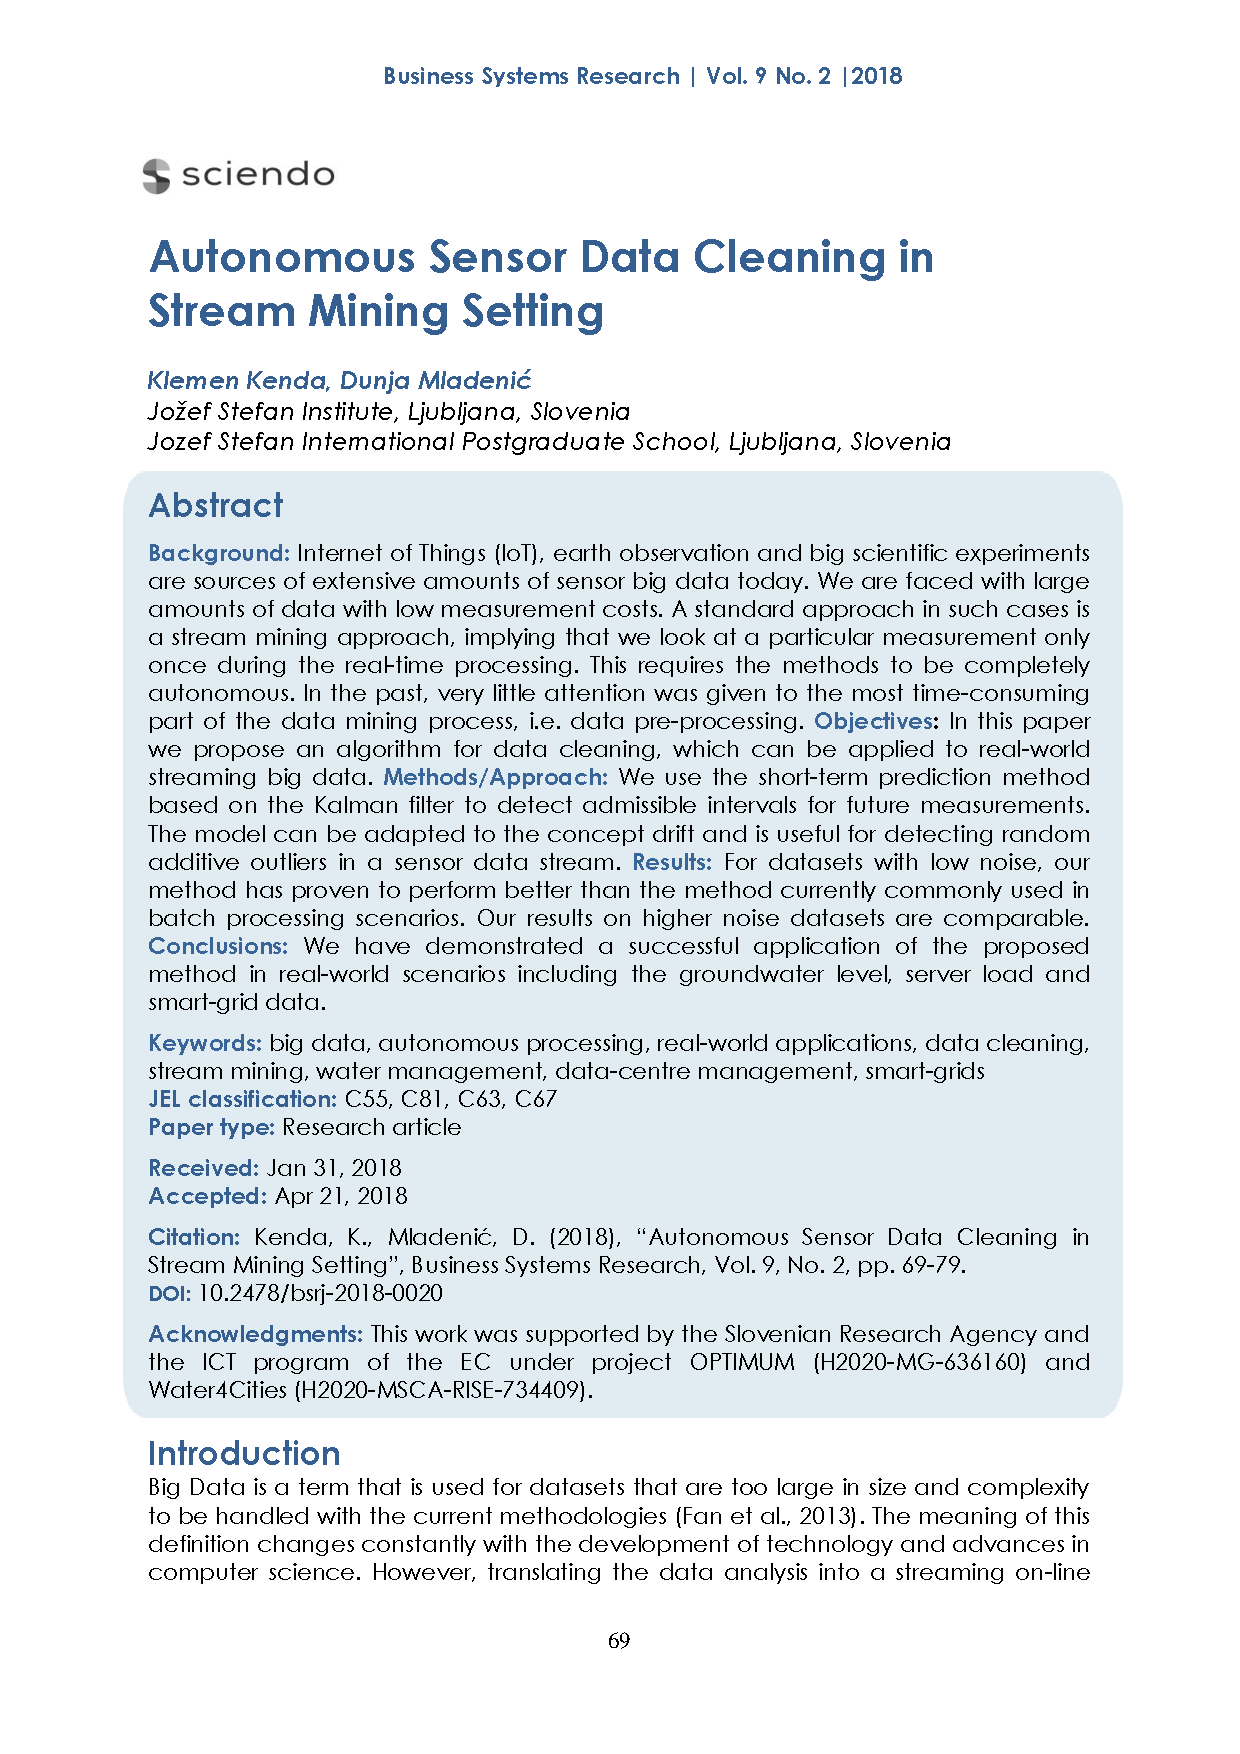
\includepdf[pages=-]{papers/data_cleaning.pdf}